% !TeX root = ../main.tex

\chapter{Hubbard Model \& Strong Coupling Perturbation Theory}

\begin{paracol}{2}
This will talk about the Hubbard model on 2D square lattice with
hopping $t_{ij} = \braket<i,j>$.
The Hamiltonian can be separated into two parts using tight-bounding model
\begin{equation}
  \mathcal H = \mathcal H_t + \mathcal H_u
= -\sum_{ij,\sigma\tau} t_{ij,\sigma\sigma'}
  c_{i\sigma\tau}^\dagger c_{j\sigma\tau}
  + \mathcal H_u
\end{equation}
where $\tau$ stands for different orbitals, like
\ce{Cu}, \ce{Ni}, \ce{Fe} have 3d orbitals,
\ce{Ru} has 4d orbitals, \ce{Ir} has 5d orbitals.
\switchcolumn \centering
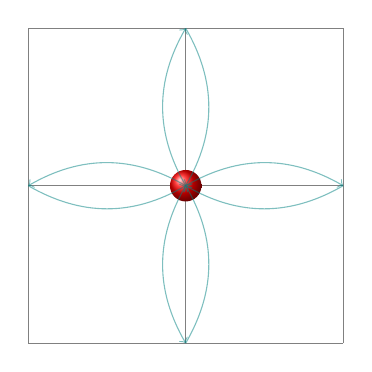
\begin{tikzpicture}[scale = 2]
  \draw [help lines] (-1,1) grid (1,-1);
  \shade [ball color = red] (0,0) circle (.1);
  \draw [->, teal, opacity = .5] (0,0) to [bend right] (-1,0);
  \draw [->, teal, opacity = .5] (0,0) to [bend left] (1,0);
  \draw [->, teal, opacity = .5] (0,0) to [bend right] (0,-1);
  \draw [->, teal, opacity = .5] (0,0) to [bend left] (0,1);
  \draw [<-, teal, opacity = .5] (0,0) to [bend left] (-1,0);
  \draw [<-, teal, opacity = .5] (0,0) to [bend right] (1,0);
  \draw [<-, teal, opacity = .5] (0,0) to [bend left] (0,-1);
  \draw [<-, teal, opacity = .5] (0,0) to [bend right] (0,1);
\end{tikzpicture}
\end{paracol}

We only take the simpliest case: 1 orbital
\begin{equation}
  \mathcal H = \mathcal H_t + \mathcal H_u
= -\sum_{ij} t_{ij} c_{i\sigma}^\dagger c_{j\sigma}
+ U \sum_i \mathemph[n_\downarrow]{n_\uparrow n_\downarrow}
\end{equation}
For the last term $n_\uparrow n_\downarrow$ in Group theory: Casimir element,
connects with all different types of orders, like Kondo coupling

\section{Symmetries of Hubbard model: SU(2)-spin}

Symmetries mean the spin operation is invariant. That is
\[
  c_\sigma' = U_{\sigma\sigma'} c_{\sigma'},
  \quad \mathcal H\big|_{\sigma\to\sigma'} = \mathcal H.
\]
In the tensor form
\[
  \sum_a \sigma_{\alpha\beta}^a \sigma_{\gamma\delta}^a
= 2\delta_{\alpha\delta} \delta_{\beta\gamma}
- \delta_{\alpha\beta} \delta_{\gamma\delta}
\]
By applying the operator basis idea
\[
  \hat {\mathbf S} = \frac12 c_\alpha^\dagger \bm\sigma_{\alpha\beta} c_\beta
\]
and the properties of Pauli matrices, one can obtain
\begin{equation}
  \sum_{\bm\gamma} (\hat {\mathbf S} (\bm r))^2
= \sum\ab(\frac34 n(\bm r) - \frac32 n_\uparrow n_\downarrow)
\end{equation}
Then the Hamiltonian becomes
\begin{equation}
  \mathcal H_n(r) = -\frac32 \hat {\mathbf S}^2 + \frac{nU}{2}.
\end{equation}
For $U(1)$-charge
\[
  c_\sigma'(\bm r) = \upe^{\iu\theta(\bm r)} = c_\sigma(\bm r)
\]
in $H_t$, $H_u$, $c^\dagger c$, the minimal coupling
\[
  -t\sum_{\braket<\bm r\bm r'>} c^\dagger(r)
  \upe^{\iu\frac{e}{hc}\int_{\bm r'}^{\bm r}\d r'' \bm A(x)} c_\sigma(\bm r')
= -t\sum_{\braket<\bm r\bm r'>} c^\dagger(r)
  \upe^{\theta(\bm r) - \theta(\bm r')} c_\sigma(\bm r')
\]
\subsection{Particle-hole system}
Special for AB-lattice: bipartite.
We have the transformations
\begin{equation}
  \begin{cases*}
    c(\bm r) \to +c^\dagger(\bm r), & if $\bm r \in A$,\\
    c(\bm r) \to -c(\bm r),  & if $\bm r \in B$
  \end{cases*}
\end{equation}
\begin{paracol}{2}
Then, we have the transformation in the hopping term
\[
  \begin{aligned}
    t c^\dagger c & \to -t c^\dagger c,\\
    c_\uparrow(\bm r) & = d_\uparrow(\bm r),\\
    c_\downarrow(\bm r) & =
    \begin{cases}
      +d_\downarrow^\dagger(\bm r),\\
      -d_\downarrow(\bm r).
    \end{cases}
  \end{aligned}
\]
\switchcolumn \centering

\includegraphics[width = \linewidth]{feynmann38.jpeg}
\end{paracol}
Then, the Hamiltonian can be transformed to
\begin{equation}
  \mathcal H(t,u) = \mathcal H(t,-u) + uN_\uparrow, \quad
  \begin{matrix}
    n_\uparrow + n_\downarrow\\
    n_\uparrow - n_\downarrow
  \end{matrix}
= d_\uparrow^\dagger d_\uparrow - d_\downarrow^\dagger d_\downarrow + 1
= S_z^d + 1
\end{equation}
Then $Q \to S_z + 1$, $S_z \to Q - 1$.
We obtain from the hole doping to the electron doping with $-t'$.
By SU(2) $\otimes$ SU(2), $U(1) \otimes U(1) = \text{SU(2)}$, we have the
operator basis
\[
  \begin{cases}
    [c, n] = -c,\\
    [c^\dagger, n] = +c,\\
    \underbrace{[c, c^\dagger]}_\text{SU(2)} = 2n - 1
  \end{cases}
\]
where satisfies the mapping
\begin{equation}
  [S^+, S^z] = +S^+,\quad
  [S^-, S^z] = -S^-,\quad
  [S^+,S^-] = 2S^z.
\end{equation}
From AFM SDW to AFM MOTT.

\section{Weak coupling limit}

The Hamiltonian
\begin{equation}
  \mathcal H_t = -t\sum_r 2(\cos k_x + \cos k_y)
  c_{k\sigma}^\dagger c_{k\sigma}.
\end{equation}
\begin{paracol}{2}
Then, the Fermi surface is the figure on the right.
Here, in the recipitical lattice $k \sim k + a$, we have vectors
\[
  G = \ab(n\frac{2\pi}{a}, \frac{2\pi}{a}m), \quad
  \ab(\frac{2\pi}{a}, 0), \quad
  \ab(0,\frac{2\pi}{a}), \quad
  \ab(\frac{2\pi}{a}, \frac{2\pi}{a}).
\]
The energy satisfies the symmetry
\[
  \epsilon(k) = -\epsilon(k + Q), \qq{where} \bm Q = \ab(\frac\pi a, \frac\pi a)
\]
\switchcolumn \vspace* \fill \centering
\begin{tikzpicture}[scale = .75]
  \draw [->] (-2,0) -- (2,0) node [below] {$k_x$};
  \draw [->] (0,-2) -- (0,2) node [right] {$k_y$};
  \draw [dashed] (-1.5,1.5) rectangle (1.5,-1.5);
  \filldraw [pattern = north east lines]
    (0,1.5)  node [left]  {$\pi$}  -- (-1.5,0) node [below] {$-\pi$} --
    (0,-1.5) node [right] {$-\pi$} -- (1.5,0)  node [below] {$\pi$}  -- cycle;
    \draw [<->] (-1.2, .3) node {$+$} -- (.3,-1.2) node {$+$};
    \draw [<->] ({-1.5/2}, {1.5/2}) node {$+$} --
      ({1.5/2},{-1.5/2}) node {$+$};
\end{tikzpicture}
\vspace* \fill
\end{paracol}
For the point $\epsilon(k_0) = 0$, we can
obtain $\epsilon(k_0 + Q) = \epsilon(k_0)$, for $k_0 = k_{F'}$.
We can always identify two vectors on the Fermi surface
\[
  k_F(i) \Leftrightarrow k_F(i;) = k_F(i) + \bm Q
\]
called the Fermi surface nesting.
\begin{paracol}{2}
  For the transformations
  \[
    k + k' \to k'' + k''', \xlongequal{\text{lattice}}
    k + k' \to k'' + k''' + G
  \]
  where $2Q = G$.
  We can write it into the Feynman diagram.
  \switchcolumn \centering
  \begin{tikzpicture}
    \begin{feynhand}
      \vertex (a) at (-.5,0);
      \vertex (b) at (+.5,0);
      \propag [fermion] (a) --++ (-.5,.5) node [left] {$k'$};
      \propag [anti fermion] (a) --++ (-.5,-.5) node [left] {$k$};
      \propag [fermion] (b) --++ (.5,.5) node [right] {$k'''$};
      \propag [anti fermion] (b) --++ (.5,-.5) node [right] {$k''$};
    \end{feynhand}
  \end{tikzpicture}
\end{paracol}

In the Fermi liquid, we have the diagrams
\begin{figure}[htbp]
  \begin{minipage}{.18\linewidth}
    \centering
    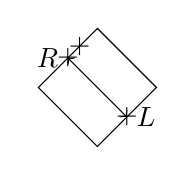
\begin{tikzpicture}[scale = .75]
      \draw (-1,0) -- (0,1) -- (1,0) -- (0,-1) -- cycle;
      \draw [<->] (-.5,.5) node [left] {$R$} node {$+$} --
        (.5,-.5) node [right] {$L$} node {$+$};
      \node at (-.3,.7) {$+$};
    \end{tikzpicture}
  \end{minipage}
  \hfill
  \begin{minipage}{.26\linewidth}
    \begin{tikzpicture}
      \begin{feynhand}
        \vertex (a) at (-.5,0);
        \vertex (b) at (+.5,0);
        \propag [fermion] (a) --++ (-.5,.5)
         node [left] {$R(2)$};
        \propag [anti fermion] (a) --++ (-.5,-.5)
         node [left] {$R(1)$};
        \propag [fermion] (b) --++ (.5,.5)
         node [right] {$R(4)$};
        \propag [anti fermion] (b) --++ (.5,-.5)
         node [right] {$R(3)$};
        \propag [photon] (a) to (b);
      \end{feynhand}
    \end{tikzpicture}
    \caption*{Forward scattering}
  \end{minipage}
  \hfill
  \begin{minipage}{.26\linewidth}
    \begin{tikzpicture}
      \begin{feynhand}
        \vertex (a) at (-.5,0);
        \vertex (b) at (+.5,0);
        \propag [fermion] (a) --++ (-.5,.5)
         node [left] {$L(2 + Q)$};
        \propag [anti fermion] (a) --++ (-.5,-.5)
         node [left] {$R(1)$};
        \propag [fermion] (b) --++ (.5,.5)
         node [right] {$R(4)$};
        \propag [anti fermion] (b) --++ (.5,-.5)
         node [right] {$L(3 - Q)$};
        \propag [photon] (a) to (b);
      \end{feynhand}
    \end{tikzpicture}
    \caption*{Backward scattering}
  \end{minipage}
  \hfill
  \begin{minipage}{.26\linewidth}
    \begin{tikzpicture}
      \begin{feynhand}
        \vertex (a) at (-.5,0);
        \vertex (b) at (+.5,0);
        \propag [fermion] (a) --++ (-.5,.5)
         node [left] {$L$};
        \propag [anti fermion] (a) --++ (-.5,-.5)
         node [left] {$R$};
        \propag [fermion] (b) --++ (.5,.5)
         node [right] {$L$};
        \propag [anti fermion] (b) --++ (.5,-.5)
         node [right] {$R$};
        \propag [photon] (a) to (b);
      \end{feynhand}
    \end{tikzpicture}
    \caption*{Unklapp}
  \end{minipage}
\end{figure}
The momentum conservation can be
\[
  (1) + (2) = (3) + (4), \quad
  (1) + (2) + Q = (3) + (4) - Q \Rightarrow
  (1) + (2) - (3) - (4) + 2Q
\]
For the nesting, the point close to $R$, von Hove singularity.
Then the Hamiltonian is
\[
  (b_L^\dagger b_L + b_R^\dagger b_R + b_{RL}^\dagger b_{LR}
+ b_{RL}^\dagger b_{RL})
\]
\begin{paracol}{2}
One can write it into a matrix
\[
  \begin{pmatrix}
    LL & RLLR\\
    RLRL & RR
  \end{pmatrix} \to \text{Gap over}
\]
with a peek in $\rho(\epsilon)$-$\epsilon$, which proportional
to $\frac{1}{4\pi^2t}\ln(t/\epsilon)$ at $\epsilon \to 0$.
\switchcolumn \centering
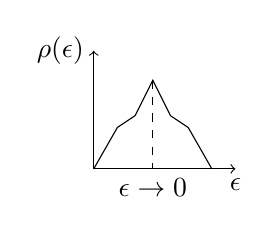
\begin{tikzpicture}[scale = .75]
  \draw [->] (0,0) --++ (2.4,0) node [below] {$\epsilon$};
  \draw [->] (0,0) --++ (0,2) node [left] {$\rho(\epsilon)$};
  \draw (0,0) -- (.4,.7) -- (.7,.9) -- (1,1.5) -- (1.3,.9) -- (1.6,.7) -- (2,0);
  \draw [dashed] (1,1.5) -- (1,0) node [below] {$\epsilon \to 0$};
\end{tikzpicture}
\end{paracol}

\section{Magnetic Instability of Fermi Liquid}

\begin{equation}
  \chi_\text{mag} = \frac1{1 - U\chi_0(S_\gamma, 0)}, \qq{if}
  1 - U\chi_0 = 0 \qq{for} q = Q_0
\end{equation}
The mean field
\begin{equation}
  \mathcal H = -t \sum_\sigma c_i^\dagger c_{j\sigma}
- \frac23 U\Sigma(\mathbf S)^2
\end{equation}
where
\[
  (\mathbf S)^2 \to \bm M(\bm r) \cdot \hat{\mathbf S(r)}
\]
Then, the mean field Hamiltonian
\begin{equation}
  \mathcal H_\text{MF} = -t \sum c_{\sigma_i}^\dagger c_{\sigma_j}
+ \sum \bm M(\bm r) \hat{\mathbf S(\bm r)}
+ \frac3{8U}  \sum_{\bm r} \bm M(\bm r)
\end{equation}
The expectation
value $\braket<\mathcal H_\text{MF}> \Leftrightarrow \braket<\mathcal H>$.
The functional derivative
\[
  \fdv{\braket<\mathcal H_\text{MF}>}{\bm M} = 0, \Leftrightarrow
  \bm M = \mathcal F(\mathcal H_\text{MF}).
\]
\begin{paracol}{2}
The neel state
\[
  \bm Q = (\pi/a, \pi/a)
\]
\switchcolumn \centering
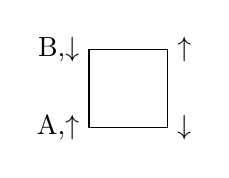
\begin{tikzpicture}
  \draw (-.5,.5) rectangle (.5,-.5);
  \node [left] at (-.5,.5) {B,$\downarrow$};
  \node [left] at (-.5,-.5) {A,$\uparrow$};
  \node [right] at (.5,.5) {$\uparrow$};
  \node [right] at (.5,-.5) {$\downarrow$};
\end{tikzpicture}
\end{paracol}
Then, the magnetic momentum
\begin{equation}
  \bm M(\bm r) = \int \d q \upe^{\iu \bm Q \cdot \bm q} \bm M(q) \to
  \bm M(\bm r) = M_0(-1)^{\bm r}
  \qq{for} \bm r \in A: (-1)^0;\ \bm r \in B, (-1)^1.
\end{equation}
Then, the mean field Hamiltonian
\begin{equation}
  \mathcal H_\text{MF} = \int \d\bm k \epsilon_k c_{k\sigma}^\dagger c_{k\sigma}
+ \int \d\bm k c_{k\alpha}^\dagger \frac12 \tau_{\alpha\beta} c_{k\beta} (k + Q)
  \cdot \frac12 M_0
  + c \cdots c_{k\beta}(k - Q) \cdot \frac12 M_0
\end{equation}
The state and the Hamiltonian in matrix
\begin{equation}
  \Psi_\sigma(\bm k) =
  \begin{pmatrix}
    c_\sigma(k)\\
    c_\sigma(k + \bar Q)
  \end{pmatrix}, \quad
  \mathcal H = \Psi_\sigma^\dagger
  \begin{pmatrix}
    \epsilon_k & \frac12\bm\tau \cdot \bm M_0\\
    \frac12\bm \tau \cdot \bm M_0 & \epsilon(k + Q)
  \end{pmatrix}\Psi_\sigma
\end{equation}
The eigen energies
\[
  E_\pm = \sqrt{\epsilon^2(k) + \frac14|M_0|^2} \qq{for} \Delta = |\bm M_0|,
  \quad
  E = \frac3{8U} |M|^2 - 2\int \d^2k E(\bm k), \qq{for} \pdv E{M_0} = 0
\]
Then, the density
\[
  \rho(\epsilon) = \frac1{4\pi^2t} \ln(t/\epsilon) + \cdots
\]
we can obtain the very small gap $\Delta = 2\pi^2t \upe^{-\sqrt{kt}/U}$,
and the parameter $|M_0| \to 0$.
The Hamiltonian
\begin{equation}
  \mathcal H  \Rightarrow L = \bar\Psi_\alpha(\iu\pdif t + \mu)
    \Psi_\alpha(\bm r, t)
  + t\Sigma(\Psi_i^\dagger\Psi_j)
  + \frac U\sigma (\bar\Psi_\sigma\tau_{\alpha\beta}\Psi_\beta)^2
\end{equation}

\subsection{Hubbard-Strantonovich-Transformation}

\begin{equation}
  \int \d\Phi
  \upe^{-\iu\ab(\frac12\Phi^2 + \lambda\bm\Phi \cdot \bm\Psi\bm\tau \Psi)}
= \text{Constant} \times \upe^{\iu\frac12\lambda(\bm\Psi\bm\tau\Psi)}
\end{equation}
We can obtain
\begin{equation}
  L' = L_0 - \sqrt{\frac U3} \vec \Phi(\bm r,t) \cdot \vec \Psi_\alpha(\bm r,t)
    \vec\tau_{\alpha\beta} \Psi(\bm r, t) - \frac12\vec\Phi^2(r,t)
\end{equation}
with $Z = \int \mathcal D\vec\Phi\mathcal D\Psi\upe^{L'}$,
the nonlinear sigma model.
\begin{equation}
  -\iu\delta(t - t') \delta_{\bm r, \bm r'} \delta_{\alpha\beta}
= (\iu\pdif t + \mu) G(\bm r, t; \bm r't'; \Phi) + t\Sigma(\epsilon_k G)
- \sqrt{\frac U3} |\vec\Phi| \bm n \cdot \bm \tau_{\alpha\gamma}
  (-1)^{x_1 + x_2} G_{\gamma\beta}(\bm r + \cdots \bar\psi)
\end{equation}
The equation for the Green's function, the $\delta$-function
\[
  -\iu\delta_{\alpha\beta}= \begin{pmatrix}
    \omega - \epsilon(k) & \sqrt{\frac U3}|\vec\Phi|\\
    -\sqrt{\frac U3}|\vec\Phi| & \omega + \epsilon(k)
  \end{pmatrix} G
\]
Then, the Green's function
\begin{equation}
  G(\bm k, \omega) = -\frac\iu
    {\omega^2 - \epsilon^2(k) + (\frac U3)|\Phi|^2}
  \begin{pmatrix}
    \omega + \epsilon(k) & \sqrt{\frac U3}|\vec\Phi|\\
    \sqrt{\frac U3}|\phi| & \omega - \epsilon(k)
  \end{pmatrix}
\end{equation}
\begin{paracol}{2}
with the energy and the gap
\[
  E(\bm k) = \sqrt{\epsilon^2 + \frac U3|\phi|^2}, \quad
  \Delta = \sqrt{U/3}|\vec\Phi|.
\]
In the figure of the gap, there is an obvious gap; after it, it will be linear.
\switchcolumn \centering
\begin{tikzpicture}
  \draw (0,0) node [left] {$u$} to [bend left = 10] (.5,.6) --++ (1,.7);
  \draw [dashed] (.5,0) --++ (0,1);
\end{tikzpicture}
\end{paracol}
Do the Schwinger-Dyson EOM.
\[
  \iu \pdif \tau G = \delta[\quad] + \cdots
+ \epsilon_k G[k,\omega] + \int \d q \quad
- \underbrace{U\braket
  <n_{i\bar\sigma} c_{i\sigma_{jj}} c_{f^{\sigma'}}^\dagger>}_
  \text{Vertex function $\Lambda$}
\]
where $U \Lambda \sim \sqrt{\frac U3} \phi(r,t) G$.
Just recall that for any case
\[
  \chi_{ab}(Q,\omega) = \frac{\chi_0}{1 - u\chi_0(Q,\omega)}.
\]
When the divergence occurs, it is a pole, which means a propagating mode.
The time-ordering $\braket<\mathcal T[S^a; S^b]>$.
The spin
\[
  \braket<n_{\bar\sigma} c_{\sigma i}; c_{\sigma'f}> \to
  \braket<nc_{\sigma i}; c_{\sigma'f}>
- U\braket<S^z c_{\sigma i}; c_{\sigma'f}>
\]
where $n + \iu S^z = \iu n_\uparrow$, $n - \iu S^z = -2n_\downarrow$.
The last term denotes the coupling between $S$ and $G$.
The propagator $S_{ab}$
\begin{equation}
  \iu\pdif t S_{ab} = \text{From $\chi_{ab}$} \Rightarrow
  S_{ab} \cong \frac{\chi_0(q,\omega)}{1 - \frac{2U}{3} \chi_0(q,\omega)}
  \cong \frac3{2U} \frac1{(q - Q)^2 + Z\omega^2}.
\end{equation}
one can break down $\chi(0,Q)$ to the denominator $(q - Q)^2 + Z\omega^2$.
The EOM
\begin{equation}
  \iu \pdif t \braket<S_i^z c_{\sigma i}; c_{\sigma' f}^\dagger>
= \braket<[S_i^z c_\sigma, \mathcal H], c_{\sigma'f}^\dagger>
\sim \braket<S_i^z S_i^z> \braket<c_{\sigma i}; c_{\sigma'}f^\dagger>
\end{equation}
\begin{paracol}{2}
Fundamentally, we will find
\begin{multline*}
  \Sigma \cong \frac{2U}{3} \int \d\omega'\d q
  G_{k-q}(\omega - \omega') \frac{2U}{3} \chi_s(q,\omega')\\
= \ab(\frac{2U}{3})^2 \int \d k' \d\omega'
  G\ab(\frac3{2U} \frac1{(q - Q)^2 + z\omega^2})
= \frac{2U}3 M_0
\end{multline*}
Coming from the bubble.
\switchcolumn \vspace*\fill \centering
\begin{tikzpicture}
  \begin{feynhand}
    \vertex (a) at (-1.5,0);
    \vertex (b) at (-.5,0);
    \vertex (c) at (+.5,0);
    \vertex (d) at (+1.5,0);
    \propag [fermion] (a) to (b);
    \propag [fermion] (c) to (d);
    \propag [photon, in = +90, out = +90] (b) to (c);
    \propag [fermion] (b) to (c);
  \end{feynhand}
\end{tikzpicture}
\vspace*\fill
\end{paracol}

\section{Strong Coupling Perturbation ($\mathsf{u \to \infty}$)}

The unsolved question: How to generate perturbation sequences?

With Gell-Mann-Low,
\[
  \upe^{\iu(\mathcal H_0 + \alpha\delta\mathcal H)t} \ket|\Psi>
\]
Usually
\[
  \upe^{\iu(A + B)} = \upe^{\iu A}\upe^{\iu B} \upe^{\iu[A,B]/2!}
  \upe^{\iu[[A,B],A]/3!} \cdots, \quad
  \upe^{\iu A}\upe^{\iu B} = \upe^{\iu(A + B) + \cdots}
\]
The equation of motion
\begin{equation}
\begin{aligned}
  O(t) &
= \upe^{\iu(H_0 + \delta H)\d t} \hat O \upe^{-\iu(H_0 + \delta u) \d t}
= \upe^{\iu \delta H\d t} \upe^{\iu H_0\d t} \hat O
  \upe^{-\iu H_0\d t} \upe^{-\iu\delta H\d t} \upe^{-\iu[H, \delta H]/2!}
  \cdots\\
& = \upe^{\iu[\quad] \d t} \upe^{\iu\delta H \d t}
  (\hat O + \iu[H_0, \hat O]\d t + \iu^2 [H_0,[H_0,\hat O]]\d t^2 \cdots)
  \upe^{\iu\delta H\d t}\upe^{\iu[\quad]}\\
& = (\hat O + \iu[H_0, \hat O]\d t + \iu[\delta H, \hat O]\d t
+ \iu[H_0,[H_0,\hat O]] + \iu^2[\delta H, [\delta H, \hat O]]\d t^2\\
& \quad + \iu^2[\delta H, [H_0, \hat O]]\d t^2
        + \iu^2[H_0,[\delta H, \hat O]]\d t^2)
+ \cdots\\
& = \hat O + \iu[H,\hat O] \d t + \frac{\iu \d t^2}{2!}([H_0,[H_0,\hat O]]
  + \alpha^1 (\quad) + \alpha^2 (\quad))
\end{aligned}
\end{equation}
The first and second orders of time-derivative
\begin{equation}
  \pdif t \hat O = \iu[H,O], \quad
  \pdif[2]t \hat O = \frac1{2!}(\qquad)
\end{equation}
We can define
\[
  H_0, \quad
  \iu\pdif t G_0 = \delta + \Lambda [\quad] \to
  \pdif[2]t G = \cdots \leftarrow G_0
\]
generate by $G_0$.
$\sum t_{ij} c^\dagger c$, $\sum c^\dagger c^\dagger cc \to b^\dagger b$

\paragraph{Complete operator basis set orthogonal}

The trace $\Tr[u^\alpha u^\beta] = \delta_{\alpha\beta}$.
\[
  \{
    c_{\sigma i}, c_{\sigma i}^\dagger,
    \eta_{\sigma i} = n_{\sigma i} - \frac12, \identity
  \}
\]
where $\eta^z = n - \frac12$, $\eta^x = (c + c^\dagger)/2$,
$\eta^y = (c - c^\dagger)/2$,
$[\eta^\alpha, \eta^\beta] = \iu \epsilon_{\alpha\beta\gamma} \eta^\gamma$,
$\{\eta^\alpha, \eta^\beta\} = \delta_{\alpha\beta}/4$.

\paragraph{Two species cons}

\begin{enumext}[columns = 2]
  \item Spin: $\delta_i^a = c_{i\alpha}^\dagger
    \tau_{\alpha\beta}^a c_{i\beta}$, charge
  $c_\uparrow c_\downarrow^\dagger; c_\uparrow, c_\downarrow$.
  \item Vertex: $v_\sigma^\dagger = c_{\sigma i}^\dagger \eta_{\bar\sigma}$,
  $v_{\sigma i} = c_{\sigma i} \eta_{\bar\sigma i}$.
  \item Casimir: $D_i = \eta_{\uparrow i} \eta_{\downarrow i}$.
  \[
    H_0 = UD: \quad
    [D_i, c_{\sigma i}] = -\hat v_{\sigma i},\quad
    [D_i, \nu_{\sigma i}] = -c_{\sigma i}/4, \quad
    [D, c^\dagger] = \nu^\dagger,\quad
    [D,\nu^+] = \frac{c^\dagger}{4}
  \]
\end{enumext}
The EOM for $G_0$
\[
  G_0 = \braket<\mathcal T[c_{\sigma i(t)_j} c_{\sigma f}(t')]>:\
  -\pdif[2]t G_0 = \frac{U^2}{4} G_0 \Rightarrow G_0
  = \frac{\braket<c_\sigma c_\sigma>(t' - t)}{\omega^2 - U^2/4}
\]
The first time derivative
\[
  \iu\pdif t G_0 = \delta(t) - U\braket<\nu; c^\dagger>
\]
The second time derivative
\[
  -\pdif[2]t G_0
= \delta'(t) + U\iu\pdif t\braket<\nu_\sigma; c_{\sigma'}^\dagger>, \quad
  \iu \pdif t\braket<\mathcal T[\nu_\sigma; c^\dagger]>
= \delta(t) \braket<[\nu_\sigma, c_{\sigma'}^\dagger]_+>_0 + \frac{U^2}{4e} G_0.
\]
Substitute the first order time-derivative to the second order time-derivative
\[
  -\pdif[2]t G_0 = \delta'(t) + U\delta_t \braket<\hat \eta_{\bar\sigma}>_0
+ \frac{U^2}{4} G_0, \Rightarrow G_{0,\sigma\sigma'}
= \frac{\omega - U\braket<\eta_{\bar\sigma}>_0}{\omega^2 - U^4/4}
= \frac{\omega - U\sigma\braket<SZ>_0}{\omega^2 - U^2/4} \delta_{\sigma\sigma'}
\]
\begin{paracol}{2}
The selection rule
\[
  \uparrow: G_{0,\sigma\sigma'} \big|_{\sigma^z = \pm\frac12}
= \frac1{\omega \pm U/2}
\]
Allowing some
arbitrary $[G] = \frac{\omega - U \bm M \cdot \bm \sigma}{\omega^2 - U^2/4}$.
\switchcolumn \centering
\[
  \begin{array}{ccc}
    & \uparrow \downarrow\\
  \uparrow & & \downarrow\\
  & 0
  \end{array}
\]
\end{paracol}
The superexchange
\[
  \braket<c_i^\dagger c_j + \text{h.c.}> = -2\Re\braket<c_ic_j^\dagger>
\]
The real part of the Green's funnction in the equal time limit
\[
  (\Re \iu)G[c_{\sigma,i}; c_{\sigma,j}](t \to 0^+)
= 2\Im G[c_ic_j^\dagger]
\]
The EOM
\begin{equation}
  -\pdif[2]t G = -tU\braket<\eta_{\bar\sigma i}^z>
    G_0[\hat c_{\sigma j}; c_{j\sigma}^\dagger]
\end{equation}
The second perturbation to $G$
\begin{equation}
  \delta G = -\frac{t U M^z(\omega - UM_j^z)}
    {\omega^2(\omega^2 - \frac{U^2}{4})}
  \xlongrightarrow{\text{Super Feynman Exchange}}
  \frac{4t^2}{U} \braket<s_i^t> \braket<s_j^z>
\end{equation}
where $\{nu_\sigma, c_{\sigma'}^\dagger\}
= \delta_{\sigma\sigma'} \eta_{\bar\sigma}$, $\eta_{\bar\sigma}
= n_{\bar\sigma} - \frac12 - m_z$.
We can write the direct product $\ket|\downarrow>\otimes \ket|\uparrow>$,
$\ket|\uparrow> \otimes \ket|\downarrow>$.
\begin{paracol}{2}
Now, we are able to get the full EOM at second order
\begin{align*}
  -\pdif[2]t G & = \iu\delta'(t) + U\iu\pdif t G[\ni_{\sigma ix_i};c_f^\dagger]
  - \sum t_{ij} (\iu\pdif t) G[c_{j\sigma}; c_f^\dagger],\\
  \iu\pdif t G[\nu_\sigma;c_f^\dagger] &
= \delta(t) \braket<\eta_{\bar\sigma}> \delta_{\sigma\sigma'}
  + \frac U4 G[c_i; c_f^\dagger]
  - \sum t_{ij} G[\eta_{\bar\sigma i} c_{j\sigma}; c_f^\dagger]\\
  & \quad + \cancel{G[S_i^\dagger c_{\bar\sigma j}; c_{\sigma f}^\dagger]}
  - \cancel{G[c_{\bar\sigma j}^\dagger c_{\sigma i}
      c_{\bar\sigma i};c_{\sigma f}^\dagger]}
\end{align*}
\switchcolumn \vspace*\fill \centering
\begin{tikzpicture}
  \begin{feynhand}
    \vertex (a) at (0,0);
    \propag [fermion] (a) --++ (-.5,.5) node [right] {$\downarrow$};
    \propag [anti fermion] (a) --++ (-.5,-.5) node [right] {$\uparrow$};
    \propag [photon] ([yshift = 1pt]a) --++ (1,0) node [right] {$S^+$};
    \propag [photon] ([yshift = -1pt]a) --++ (1,0);
  \end{feynhand}
\end{tikzpicture}
\vspace*\fill
\end{paracol}
Finally,
\begin{equation}
  (\omega^2 - \frac{U^2}{4}) G
+ \sum t_{ij} (\omega + U m_z (-1)^{\bm x_i} + \bm e_j)G
= \omega + U m_z \sigma
\end{equation}
Do the Fourier Transformation
\begin{multline}
  \ab(\omega^2 - \frac{U}{4} - \omega \epsilon_k) G[k_i, k_f]
- U m_z' \epsilon_{k-Q} G[k_i - Q, k_f]
= \ab(\omega - \sigma^2 m_z \frac U2) \delta_{\bm k_i, \bm k_f}\\
\Rightarrow
  \begin{pmatrix}
    \omega^2 - \frac{U^2}{4} - \omega \epsilon_k & -\sigma m_z U\epsilon_k\\
    -\sigma U m_z \epsilon_k & \omega - \frac{U^4}{4} + \omega\epsilon_k
  \end{pmatrix}
  \begin{pmatrix}
    G_{kk} & G_{kQ}\\
    G_{k, \iu Q} & G_{QQ}
  \end{pmatrix} =
  \begin{pmatrix}
    \omega - \sigma U/2 & 0\\
    0 & \omega t + \sigma U/2
  \end{pmatrix}
\end{multline}
where $\epsilon_{k-Q} = -\epsilon_k$.
Then
\begin{equation}
  G[k,k]
= \frac{\ab(\omega - \sigma m_z U/2)
        \ab(\omega^2 - \frac{U^2}{4} - \epsilon_k \omega)}
       {\ab(\omega^2 - \frac{U^2}{4})^2
        - \epsilon_k^2 m_z^2 U^2 - \epsilon_k^2 \omega^2}
\end{equation}
For $i = 1$, $\ldots\,$,~$4$, we can obtain
\begin{equation}
  \omega_{0,i} = \pm \frac U2
    \sqrt{1 + \tilde \epsilon_k^2 \pm |\tilde \epsilon_k|
      \sqrt{\tilde\epsilon_k^2 + 2(1 - Am_z^2)}}.
\end{equation}
$\tilde \epsilon_k = \sqrt2\epsilon_k/m$ is the normalized dispersion.
We obtain the band-flipping. The flat band is a non-trivial flat band.
One cannot hop a spin-down to spin-down, so this is a perfect Bloch reflection
in a flat band.

We wang to do a thermal
\[
  A\ket*|
  \begin{matrix}
    \uparrow & \downarrow\\
    \downarrow & \uparrow
  \end{matrix}>, \quad
  B \ket*|
  \begin{matrix}
    \downarrow & \uparrow\\
    \uparrow & \downarrow
  \end{matrix}>.
\]
This is introduced in RVDS
\[
  \braket<S_i^\dagger S_j^\dagger>
  (\sim \braket<|s|c_{i\uparrow}^\dagger c_{j\downarrow}^\dagger
    c_{i\uparrow c_{j\downarrow}}>\ \text{incoherent copper pair})
  + \braket<s_i^\dagger s_j^\dagger>.
\]
For pure spinate, we have $\braket<s_i^z s_j^z>$.
This RVB correction can be factored out $[s_i^\dagger s_j^-, H_t + H_t]$.
\begin{center}
  
\includegraphics[width = \linewidth]{feynmann39.jpeg}
\end{center}

\section{Kondo Problem}

Starting from the resistivity from impurity scattering: impurities on
\ce{Au} films, \ce{Zn} films, \ce{Fe}, \ce{Ni}, \ce{Mn}, or \ce{Cu} films.
\begin{paracol}{2}
The behaviors of the resistivity can be tuned by the thickness of the films.
\begin{enumext}
  \item 2D: the resistivity usually goes up as $T$ decreases, and
  sometimes diverge.
  \item Or get stable at low $T$, or decreases.
\end{enumext}
Sometimes, $R(T)$ has a minimum, then $R(T) - R(0) \sim T^2$.
\switchcolumn
\begin{figure}[htbp]
  \centering
  \begin{tikzpicture}
    \draw [->] (0,0) -- (3,0) node [below] {$T$};
    \draw [->] (0,0) -- (0,3) node [left] {$R(T)$};
    \draw [->] (3,1) -- (2,1) to [bend left] (.7,3);
    \draw (3,1) -- (2,1) to [bend left] (.2,3);
    \draw [rounded corners = 20pt] (3,1) -- (2,1) -- (1,1.5) -- (0,1.5);
    \draw [rounded corners = 20pt] (3,1) -- (2,1) -- (0,.2);
    \draw [rounded corners = 20pt, orange]
      (3,2.8) -- (2.6,2.6) -- (1.5,.8) -- (.5,2.5) -- (0,3);
    \fill [pattern = north east lines] (.5,2.3) -- (1.5,1) -- (2.5,2) -- cycle;
  \end{tikzpicture}
  \caption{$R(T) - T$}
  \label{fig:kondo_temperature}
\end{figure}
\end{paracol}
In magnetic impurity systems
\begin{enumext}
  \item Magnetic suscbility: $\psi_m$. Curie-weiss $T \ll T_F$.
  $g$-factor: \~ isolated magnetic impurity atoms.

  At very low $T$ (Kondo temperature $T_K$): the
  magnetibility $\sim \log(T/T_k)$.
  \[
    \chi(0) \sim n_\text{imp}/T_k, \quad
    \chi(T) - \chi(0) \sim -T^2.
  \]
  \item $R(T)$: The minimum $R(T) - R(0) \sim T^2$, $R(0) \sim$ unitairy
  limit (maximum).
  \item Entropy: specific heat in this case.
  \[
    \int \d \tau C_V(T)/T, \quad
    S_e \sim \pdv S\mu \sim \pdv Sn
  \]
  Entropy release at $T_k$: Only include magnetic entropy.
  For $H = -B_zS^z$, the magnetic density $\rho = \upe^{-S^z/k_BT}$
  The spin
  \[
    \begin{cases*}
      \ketbra|\uparrow><\uparrow| + \ket|\downarrow><\downarrow|\\
      \ketbra|\uparrow><\uparrow| & Fermi sea: $f(\epsilon, T)$,
      see the behavior $C_V/T \sim \nu$.
    \end{cases*}
  \]
\end{enumext}
The questions are
\begin{enumext}
  \item $T_k \ll T \ll T_F$, local momentum formation.
  Basically, the local momentum formation is in the center
  of~\ref{fig:kondo_temperature}.
  \item Near the $T_k$: $\log(T/T_k)$, crossover.
  \item Below $T_k$: local moment get ``screened''.
  \item Why $R(T)$ can decrease, belongs to Kondo lattice.
\end{enumext}

\subsection{Local moment Formation (Charge pseudo-spin):
  $\mathsf s$-$\mathsf d$ exchange}

This case has to deal with \emph{Anderson impurity model},
$T < \Delta E \sim U$.
$s$ is the orbital, $d$ is the impurity.
The Hamiltonian
\[
  \mathcal H = \sum_{k,\sigma} \epsilon_k n_{k\sigma}
    + \sum_{k\sigma}(V(\bm k) C_{k\sigma}^\dagger f_\sigma
    + V^*(k) f_\sigma^* c_{k\sigma})
    + \underbrace{E_f n_f + U n_{f\uparrow} n_{f\downarrow}}_
      \text{atomic}
\]
Atomic limit
\[
  \begin{cases}
    \ket|f^2> & E(f^2) = 2E_f + U,\\
    \ket|f^0> & 0,\\
    \ket|f'\uparrow>,\ \ket|f'\downarrow> &
    E_f.
  \end{cases}
\]
\begin{paracol}{2}
Transformation between states
\[
  \Delta E = \frac U2 \pm (E_f + \frac U2).
\]
$U$-interaction should be
\[
  \frac U2 > \ab|E_f + \frac U2|
\]
Using the half-$U$ approximation for convenience to deal with.
Doubly occupied $\uparrow\downarrow$: Valence fluctuation kondo.
\switchcolumn \centering
\begin{tikzpicture}
  \draw [->] (-2.5,0) -- (3,0) node [below] {$U$}
   node [above] at (1.5,0) {Local moment};
  \draw [->] (0,-2) -- (0,2) node [left] {$E_f + \frac U2$};
  \draw (2.5,2) -- (0,0) -- (2.5,-2);
  \fill [pattern = north east lines] (2.5,2) -- (0,0) -- (2.5,-2);
  \node [above] at (-1,0) {$f^0 = f^2i$};
  \node [below] at (-1,0) {Charge Kondo};
\end{tikzpicture}
\end{paracol}
From SWT, ``integrate out'', ``renormalization
the Hamiltonian becomes
\[
  H = \sum \epsilon_k n_{k\sigma} + J_k \vec S_{i=0} \cdot \vec S,\quad
  \vec S_b = c_{0\alpha}^\dagger \bm \sigma_{\alpha\beta} \hat c_{0\beta},
  \quad \vec s = f_\alpha^* \bm \sigma_{\alpha\beta} f_\beta, \quad J_k = V
\]
At the impurity, it has two electrons.

\subsection{Kondo's solution to $R$ minimum}

\paragraph{Resistivity \& scattering theory}

\begin{example}[$T$-matrix]
  The Green function
  \[
    G = G_0 + G_0 \hat T G, \quad
    T = \frac{V}{1 - G_0V}, \quad
    \begin{tikzpicture}[baseline = -3pt]
      \begin{feynhand}
        \propag [fermion] (0,1pt) to (1,1pt);
        \propag [fermion] (0,-1pt) to (1,-1pt);
        \propag [fermion] (1,0) node {$\times$} to (2,0);
      \end{feynhand}
    \end{tikzpicture} +
    \begin{tikzpicture}[baseline = -3pt]
      \begin{feynhand}
        \propag [fermion] (0,0) to (1,0) node {$\times$};
        \propag [fermion] (1,0) to (2,0) node {$\times$};
        \propag [fermion] (2,0) to (3,0);
      \end{feynhand}
    \end{tikzpicture} \cdots
  \]
  which can be expressed in a Feynman diagram. One can obtain
  \[
    G = \frac{G_0}{1 - G_0T}
      = \frac{1}{G_0^{-1} - G_0TG_0^{-1}}\\
      \xlongequal{G_0^{-1}=\omega-\epsilon_k}
        \frac{1}{\omega - \epsilon_k - \Sigma} = \frac1{\omega - \epsilon_k^*}
      + \iu\frac\hbar2 \Sigma^{-1}(k,\omega)
  \]
  The imagine part
  \[
    \Im\Sigma(k,\epsilon_k) = C_\text{impurity density}
    \Im(\braket<k|\hat T(\epsilon_k)|k>) = -C_\text{imp} \frac{k}{2m} \sigma(k)
  \]
  The $\sigma(k)$ here is not conductivity, it is a cross-sectioin.
  The relaxation time
  \[
    \tau^{-1}(k) = c_\text{imp} v_k \sigma(k)
  \]
  In the Boltzmann equation, the relaxation time approximation
  \[
    \frac1{\tau(k)} = 2\pi C_\text{imp}
    \int \d k' |T_{kk'}|^2 \delta(\epsilon(k) \epsilon(k')) (1 - \cos\theta')
  = \bm k \cdot \bm k'
  \]
  Scattering phase shift enhance the back scattering, cause Anderson
  localization.
\end{example}

\paragraph{Linear response \& Kondo formula}

\[
  \frac{\braket<\bm j(\omega, T, \bm E)>}{\bm E} \bigg|_{\bm E \to 0} = [\sigma]
\]
where $\bm E$ is not parallel to $\bm j$. Then,
\[
  [\sigma] \bm E = \bm j,\quad [\sigma] = \begin{pmatrix}
    \sigma_{xx} & \sigma_{xy}\\
    \sigma_{yx} & \sigma_{yy}
  \end{pmatrix}
\]
with $\sigma_{xy} = -\sigma_{yx}$. The microscopic
\[
  \pdv\rho t - \nabla\cdot \bm j = 0, \quad
  \pdv{\hat \rho}t = \iu[H,\hat \rho], \quad
  \pdv{\hat \rho_c}t = \iu[H_0, \sum_\sigma n_{iu\sigma}]
\]
\begin{paracol}{2}
One can calculate
\begin{align*}
    \bm j & = \sum \pdif{\bm k} \epsilon_k c_k^\dagger c_k
  = \braket<\pdif{\bm k} \epsilon_k c_k^\dagger c_k>, \\
    \fdv{j_\alpha}{E^b} &
  = \fdv*{\braket<\pdif a\epsilon_k c_k^\dagger c_k>}{E^b}
  = \fdv*{\sum_k \pdif a\epsilon_k G[k,\omega]}{E^b}\\
& = \braket<\bm j_a; \bm j_b(1 + \Gamma \cdots)>
\end{align*}
\switchcolumn \centering
\begin{tikzpicture}
  \begin{feynhand}
    \vertex (a) at (0,0);
    \vertex (b) at (2,0);
    \propag [fermion] (a) to[in = 105, out = 75]
     node [near end, above] {$c_k$}
     node [near start, above] {$c_k^\dagger$} (b);
    \propag [fermion] (b) to[in = -75, out = -105]
     node [near start, below] {$c_k^\dagger$}
     node [near end, below] {$c_k$} (a);
    \node [left]  at (a) {$\nu_a = \pdif{k_a}\epsilon_k$};
    \node [right] at (b) {$\nu_b = \pdif{k_b}\epsilon_k$};
    \fill [pattern = north east lines] (1.6,.5) -- (1.6,-.5) -- (2,0) -- cycle;
  \end{feynhand}
\end{tikzpicture}
\end{paracol}
\[
  J_k \vec S_0 \cdot \vec s_f = J_k^z s_0^z s_f^z
+ J_z^+ (s_0^+s_f^- + S_0^- s_f^+)
\]
SU(2): Anisotropy can tune/control the process. We only need to compute
\[
  \braket<k',\uparrow|T(\epsilon^+)|k,\uparrow>_{(2)}
\]
to the second order. In diagram
\begin{center}
  \begin{minipage}{.48\linewidth}
    \centering
    \begin{tikzpicture}
      \begin{feynhand}
        \propag[fermion] (-1.5,1) node [left] {$k\uparrow$} to (-.5,0)
         to [in = 75, out = 105] node [above] {$k_2\downarrow$} (.5,0)
         to (1.5,1) node [right] {$k'\uparrow$};
        \propag [chasca] (-1.5,0) to node [below] {$\downarrow$} (-.5,0);
        \propag [chasca] (-.5,0) to node [below] {$\uparrow$} (.5,0);
        \propag [chasca] (.5,0) to node [below] {$\downarrow$} (+1.5,0);
      \end{feynhand}
    \end{tikzpicture}
  \end{minipage}
  \hspace*\fill
  \begin{minipage}{.48\linewidth}
    \centering
    \begin{tikzpicture}
      \begin{feynhand}
        \propag [fermion] (-1.5,1) to [out = 0, in = 120]
         node [near start, above] {$k\uparrow$} (.5,0);
        \propag [fermion] (-.5,0) to [out = 60, in = 180]
         node [near end, above] {$k'\uparrow$} (1.5,1);
        \propag [fermion] (-.5,0) to [out = 90, in = 90]
         node [below] {$k_2\downarrow$} (.5,0);
        \propag [chasca] (-1.5,0) to node [below] {$\uparrow$} (-.5,0);
        \propag [antsca] (-.5,0) node [below] {$s^-$} to (.5,0);
        \propag [chasca] (.5,0) node [below] {$s^+$} to
         node [below] {$\uparrow$} (+1.5,0);
      \end{feynhand}
    \end{tikzpicture}
  \end{minipage}
\end{center}
\[
  g(\epsilon)
= \frac1{N_s} \sum_k \frac{f(\epsilon_0)}{\epsilon_k - \epsilon - \iu S}; \quad
  \tau^{-1}(k) \propto \frac{c_\text{imp}}{\epsilon_F}
    [1 - 2J(g(\epsilon_k) + g^*(\epsilon_k))]
\]
The resistance
\[
  R_\text{imp}^\text{spin}
= \frac{3\pi m T^2s(s + 1)}{2\upe^2\epsilon_F^*}
  (1 - 4J\rho_0(\epsilon_F) \ln(k_BT/D))
\]
For $R(T) = aT^5 + c_\text{imp}R_0 - c_\text{imp} R_1 \ln(k_BT/D)$,
the functional derivative
\[
  \fdv{R(T)}T = 0, \Rightarrow T_{\min}
= \ab(\frac{R_1}{5a})^{1/5} c_\text{imp}^{1/5}
\]

\subsection{Logarithms divergence in observables of finite $\mathsf T$}

\begin{center}
  \begin{tikzpicture}
    \begin{feynhand}
      \propag [fermion] (-1,.5) to [out = -90, in = -90] (1,.5);
      \propag [fermion] (1,.5)  to [out = 90, in = 90] (3,.5);
      \propag [fermion] (3,.5)  to [out = -90, in = -90] (5,.5);
      \propag [fermion] (5,.5)  to [out = 90, in = 90] (7,.5);
    \end{feynhand}
    \begin{feynhand}
      \propag [chasca] (-1,.25) to [out = 90, in = 90] (1,.25);
      \propag [chasca] (1,.25) to [out = -90, in = -90] (3,.25);
      \propag [chasca] (3,.25) to [out = 90, in = 90] (5,.25);
      \propag [chasca] (5,.25) to [out = -90, in = -90] (7,.25);
    \end{feynhand}
  \end{tikzpicture}
\end{center}
\begin{gather}
  C_{\nu,\text{imp}} \sim \frac{1}{(1 + 2J\rho_0\ln(k_BT/D))^4}\\
  S_\text{imp} \sim k_B\ln(2s + 1)
    - \frac1{(1 + 2J\rho_0(\epsilon_F)\ln(k_BT/D))^3},\\
  R_\text{imp} = \frac{R_c}{2}
    \ab(1 - \frac{\ln T/T_k}{((\ln(T/T_k))^2 + \pi^2 s(s + 1))^{1/2}})
\end{gather}
$k_BT_k \sim D\upe^{-\frac12 J_k\rho_0}$.

\paragraph{Analysis Kondo exchange}

\[
  J_k \vec S_0 \cdot \vec s \to \sum_{i = x,u,z} J_i S_0^i s^i
\]
contribute to energy
\begin{equation}
  \sum_i \braket<J_i S_0^i s^i>_{(a),(b)}
= \sum s_{ab}^k s_{\alpha\beta}^k
  \ab(\frac12 J(T) \sum\frac{J_iJ_j}{t^2} |\epsilon_{ijk}|^2)
\end{equation}
From which we can obtain
\[
  J_k + \delta J_k = \braket<\quad>
= J_k + \frac1{2\pi} \frac\Gamma{t^2} \ln \frac WT \sum_{ij} J_i J_j
  |\epsilon_{ijk}|^2
\]
The components
\[
  \delta J_x = \frac{\Gamma}{2t^2}\ln\frac WT J_yJ_z,\quad
  \delta J_y = \frac{\Gamma}{2t^2}\ln\frac WT J_zJ_x,\quad
  \delta J_z = \frac{\Gamma}{2t^2}\ln\frac WT J_xJ_y.
\]
For $J_x = J_y = J_z$, then
\[
  \delta J = \frac{\Gamma}{\pi t^2} J^2 \ln \frac W{T_k}, \quad
  T_k = W\exp\ab(-\frac{\pi t^2}{\Gamma J}).
\]
\paragraph{Anderson's poorman's scaling}

The functionals $J_z[W(\lambda)]$, $J_+[W(\lambda)]$: $W(\lambda) = W/\lambda$.
\[
  J_z[W(\lambda)] = J_z[W] + \frac\Gamma{\pi t^2} J_+^2[W] \ln\lambda,\quad
  J_+[\quad] = J_+[W] + \frac\Gamma{\pi t^2} J_+z2[\quad] J_z[\quad],
\]
where $\lambda = \upe^5$, $\odv{j_z(s)}/s = 2J_+^2[s]$,
$\odv{J_+}s = 2j_+(s)j_z(s)$, $J \sim \frac1{T_1 - T_k}$.

\subsection{Strong coupling limit}

\[
  H_+ = \sum_{k,\sigma} \epsilon_k n_{k\sigma},\quad
  H_k = J_k \vec S_0 \cdot \vec s.
\]
For the new $T \to 0$, $\ket|\Psi_{0,H_t}>
  = \fbox{\tikz[baseline = -.25cm]{\begin{feynhand}
    \vertex [NWblob] at (2,0) {};
  \end{feynhand}}}$.
\[
  \delta H_t = \sum_k \delta f(\epsilon_k) \epsilon_k n_k
= \sum_{k_F} \delta(k - k_F) \delta\epsilon_k c_{k\sigma}^\dagger c_{k\sigma}
\]
where $\delta(k - k_F) \sim \delta\epsilon$,
$\delta\epsilon_k \sim \frac1m (k - k_F)$.
$\delta\epsilon \ll J_k$, $\delta\epsilon\rho_0 \Leftrightarrow J_k$.
So, the unperturbed Hamiltonian should be
\[
  \tilde H_0 = J_k \vec S \cdot \vec s
  \begin{cases*}
    \ket|\uparrow\uparrow>, \ket|\uparrow\downarrow> + \ket|\downarrow\uparrow>,
    \ket|\downarrow>, & Triplet: $E > 0$\\
    \ket|\uparrow\downarrow> - \ket|\downarrow\uparrow> & Singlet: $-E < 0$.
  \end{cases*}
\]
Then, its derivative
\[
  \delta H_t = \sum_{k\in k_F} \delta \epsilon_k c_k^\dagger c_k,
  \quad \delta\epsilon_k \sim \frac{(k - k_F)k_F}{m^*}.
\]
\[
  \vec s_0 = c_{0\alpha}^\dagger \sigma_{\alpha\beta} c_{0\beta}
= \sum_k c_{k\alpha}^\dagger \sigma_{\alpha\beta} c_{k\beta}
\]
with $\delta H_t$ as pert.
THese calculations are called the scattering problem with a bound state:
Fano resonance Kondo.
\begin{enumerate}
  \item $T_k \ll T \ll T_f$: week coupling limit, the ground state
  $\ket|\uparrow>$, $J_k \vec S_0 \cdot \vec S$.
  \item $T \sim T_k$: near the strong coupling limit, the ground state
  $\braket<\vec S_0 \cdot \vec S>(T)$: Kondo singlet formation.
\end{enumerate}
Finally, from the ground state of $T \sim T_k$, we get the saturate
unitary limit.
\begin{center}
  
\includegraphics[width = \linewidth]{feynmann40}
\end{center}
\vfill
\begin{framed}
  \centering \scshape
  Congratulations! U have reach the terminal of this course!
\end{framed}